\documentclass[12pt,a4paper]{article}

\usepackage[utf8]{inputenc}
\usepackage[T2A]{fontenc}
\usepackage[ukrainian]{babel}

\usepackage{geometry}
\geometry{left=2cm,right=2cm,top=2cm,bottom=2cm}

\usepackage{graphicx}
\usepackage{array,multirow}
\usepackage{booktabs}
\usepackage{caption}
\renewcommand{\thetable}{№\arabic{table}}
\captionsetup[table]{name=Таблиця}

\usepackage{amsmath}
\usepackage{pdflscape}
\usepackage{xcolor}

\usepackage{minted}

\usemintedstyle{friendly} % або monokai / vs / colorful
\setminted{linenos, breaklines, frame=single, fontsize=\small}

\usepackage{hyperref}

\begin{document}

    \begin{titlepage}

        % Картинка шапки (по центру, з відступом від верху)
        \begin{center}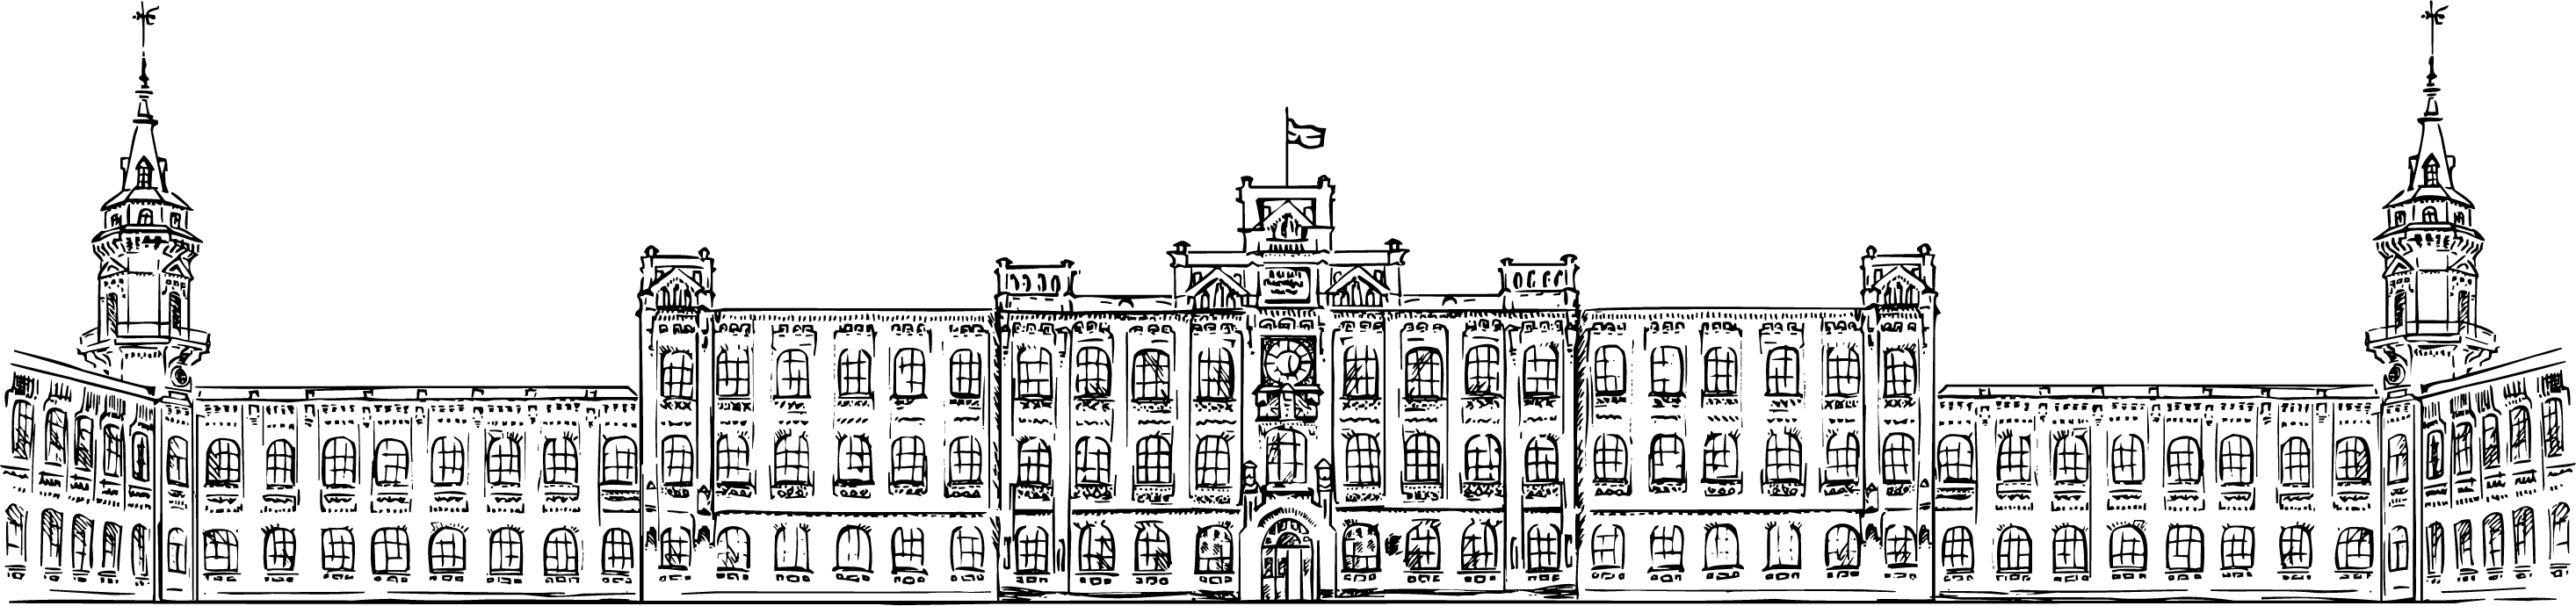
\includegraphics[width=0.7\textwidth]{../../../../TITLES/letterhead.png}\end{center}

        \begin{center}
            \large Національний технічний університет України\\
            «Київський політехнічний інститут імені Ігоря Сікорського»\\[1em]
            Факультет інформатики та обчислювальної техніки\\
            Кафедра обчислювальної техніки
        \end{center}

        \vfill

        \begin{center}
            \textbf{\LARGE Вступ до операційної системи Linux. Курсова робота}\\[2.5em]
            \textbf{\Large Практична робота №2}\\[1em]
            «Розроблення Makefile та CMake файлiв»
        \end{center}

        \vfill

        \begin{flushright}
            Виконав: студент 2 курсу ФІОТ, гр. ІО-41\\
            \textit{Давидчук А.~М.}\\[1em]
            Перевірив: \textit{Нікольський С.~С.}
        \end{flushright}

        \vfill

        \begin{center}Київ --- 2025\end{center}

    \end{titlepage}

    % Основний документ:

    \setlength{\parindent}{0em}

    \textbf{\underline{Тема:}} «Розроблення Makefile та CMake файлiв».
    
    \vspace{1em}

    \begin{center} \textbf{\Large Практична частина} \end{center}

    Використовуватиму минулий репозиторiй iз лабораторної роботи №2 (практична робота №1):
    \begin{minted}{bash}
PS C:\Users\artem\OneDrive\Desktop\coursework-calculator-lab2-3> git log --oneline
2bcb78d (HEAD -> master, origin/master, origin/HEAD) new function: Div
1fa8ece add a multiplication operation
56d74f3 improve calculation accuracy and fix truncation error
976f691 add a subtraction operation
f03784b add header guard
9972170 basic implementation
75c0e7c Initial commit
    \end{minted}

    Тут створю основний файл програми main.cpp:

    \begin{minted}{cpp}
#include <iostream>
#include "calculator.h"

int main() {
    Calculator c;
    std::cout << "2 + 3 = " << c.Add(2, 3) << "\n";
    std::cout << "5 - 1 = " << c.Sub(5, 1) << "\n";
    std::cout << "4 * 2 = " << c.Mul(4, 2) << "\n";
    std::cout << "9 / 3 = " << c.Div(9, 3) << "\n";

    return 0;
}
    \end{minted}

    А також файл CMakeLists.txt:

    \begin{minted}{text}
cmake_minimum_required(VERSION 3.10)
project(calculator_project LANGUAGES CXX)

set(CMAKE_CXX_STANDARD 11)
set(CMAKE_CXX_STANDARD_REQUIRED ON)

# Output directories
set(CMAKE_RUNTIME_OUTPUT_DIRECTORY ${CMAKE_BINARY_DIR}/bin)
set(CMAKE_ARCHIVE_OUTPUT_DIRECTORY ${CMAKE_BINARY_DIR}/lib)

add_library(calculator STATIC
    calculator.cpp
)
target_include_directories(calculator PUBLIC include)

add_executable(calc_app
    main.cpp
)
target_link_libraries(calc_app PRIVATE calculator)
    \end{minted}

    I разом iз ним файл Makefile:

    \begin{minted}{text}
# Makefile для MSVC

CC=cl
AR=lib
CFLAGS=/nologo /W4 /O2 /EHsc /I.
LDFLAGS=/nologo

OUTDIR=build
BINDIR=$(OUTDIR)\bin
LIBDIR=$(OUTDIR)\lib
OBJDIR=$(OUTDIR)\obj

APP=$(BINDIR)\calc_app.exe
LIB=$(LIBDIR)\calculator.lib

.PHONY: all clean dirs

all: dirs $(APP)

dirs:
	if not exist $(OUTDIR) mkdir $(OUTDIR)
	if not exist $(BINDIR) mkdir $(BINDIR)
	if not exist $(LIBDIR) mkdir $(LIBDIR)
	if not exist $(OBJDIR) mkdir $(OBJDIR)

$(OBJDIR)\calculator.obj: calculator.cpp calculator.h
	$(CC) $(CFLAGS) /c calculator.cpp /Fo$(OBJDIR)\calculator.obj

$(LIB): $(OBJDIR)\calculator.obj | dirs
	$(AR) /nologo /OUT:$(LIB) $(OBJDIR)\calculator.obj

$(OBJDIR)\main.obj: main.cpp calculator.h
	$(CC) $(CFLAGS) /c main.cpp /Fo$(OBJDIR)\main.obj

$(APP): $(OBJDIR)\main.obj $(LIB) | dirs
	$(CC) $(LDFLAGS) $(OBJDIR)\main.obj $(LIB) /Fe$(APP)

clean:
	- del /Q /F $(OBJDIR)\*.obj 2>nul
	- del /Q /F $(LIB) 2>nul
	- del /Q /F $(APP) 2>nul
	- rmdir /S /Q $(OUTDIR) 2>nul
    \end{minted}

    Звiдси маю таку структуру робочої областi:

    \begin{minted}{text}
PS C:\Users\artem\OneDrive\Desktop\coursework-calculator-lab2-3> tree /f
Folder PATH listing
Volume serial number is 7667-D297
C:.
    calculator.cpp
    calculator.h
    CMakeLists.txt
    main.cpp
    Makefile

No subfolders exist
    \end{minted}

    Збiрка проєкту виконується на основi CMakeLists.txt з використанням системи збирання
Ninja:

    \begin{minted}{text}
PS C:\Users\artem\OneDrive\Desktop\coursework-calculator-lab2-3> cmake -S . -B build-ninja -G Ninja -DCMAKE_BUILD_TYPE=Release
-- The CXX compiler identification is GNU 13.2.0
-- Detecting CXX compiler ABI info
-- Detecting CXX compiler ABI info - done
-- Check for working CXX compiler: C:/Strawberry/c/bin/c++.exe - skipped
-- Detecting CXX compile features
-- Detecting CXX compile features - done
-- Configuring done (1.0s)
-- Generating done (0.0s)
-- Build files have been written to: C:/Users/artem/OneDrive/Desktop/coursework-calculator-lab2-3/build-ninja
PS C:\Users\artem\OneDrive\Desktop\coursework-calculator-lab2-3> ninja -C build-ninja
ninja: Entering directory `build-ninja`
[4/4] Linking CXX executable bin\calc_app.exe
    \end{minted}

    I запускаю отриману програму:

    \begin{minted}{text}
PS C:\Users\artem\OneDrive\Desktop\coursework-calculator-lab2-3> build-ninja\bin\calc_app.exe
2 + 3 = 5
5 - 1 = 4
4 * 2 = 8
9 / 3 = 3
    \end{minted}

    Що свiдчить про успiшнiсть збiрки. Робоча область тепер має таку структуру:

    \begin{minted}{text}
PS C:\Users\artem\OneDrive\Desktop\coursework-calculator-lab2-3> tree /f /a
Folder PATH listing
Volume serial number is 7667-D297
C:.
|    calculator.cpp
|    calculator.h
|    CMakeLists.txt
|    main.cpp
|    Makefile
|
\---build-ninja
    |    .ninja_deps
    |    .ninja_log
    |    build.ninja
    |    CMakeCache.txt
    |    cmake_install.cmake
    |
    +---bin
    |       calc_app.exe
    |
    +---CMakeFiles
    |   |   cmake.check_cache
    |   |   CMakeConfigureLog.yaml
    |   |   rules.ninja
    |   |   TargetDirectories.txt
    |   |
        +---3.29.2
    |   |   |   CMakeCXXCompiler.cmake
    |   |   |   CMakeDetermineCompilerABI_CXX.bin
    |   |   |   CMakeRCCompiler.cmake
    |   |   |   CMakeSystem.cmake
    |   |   |
    |   |   \---CompilerIdCXX
    |   |       |   a.exe
    |   |       |   CMakeCXXCompilerId.cpp
    |   |       |
    |   |       \---tmp
    |   +---calculator.dir
    |   |       calculator.cpp.obj
    |   |
    |   +---calc_app.dir
    |   |       main.cpp.obj
    |   |
    |   +---CMakeScratch
    |   \---pkgRedirects
    \---lib
        libcalculator.a
    \end{minted}

    Також можемо очистити всi артефакти командою \texttt{ninja -C build-ninja -t clean}:

    \begin{minted}{text}
PS C:\Users\artem\OneDrive\Desktop\coursework-calculator-lab2-3> ninja -C build-ninja -t clean
Cleaning... 4 files.
PS C:\Users\artem\OneDrive\Desktop\coursework-calculator-lab2-3> tree /F /a
Folder PATH listing
Volume serial number is 7667-D297

C:.
|   calculator.cpp
|   calculator.h
|   CMakeLists.txt
|   main.cpp
|   Makefile
|
\---build-ninja
|   |   .ninja_deps
|   |   .ninja_log
|   |   build.ninja
|   |   CMakeCache.txt
|   |   cmake_install.cmake
|   |
|   +---bin
|   +---CMakeFiles
|   |   |   cmake.check_cache
|   |   |   CMakeConfigureLog.yaml
|   |   |   rules.ninja
|   |   |   TargetDirectories.txt
|   |   |
|   |   +---3.29.2
|   |       |   CMakeCXXCompiler.cmake
|   |       |   CMakeDetermineCompilerABI_CXX.bin
|   |       |   CMakeRCCompiler.cmake
|   |       |   CMakeSystem.cmake
|   |       |
|   |       \---CompilerIdCXX
|   |           |   a.exe
|   |           |   CMakeCXXCompilerId.cpp
|   |           |
|   |           \---tmp
|   |
|   +---calculator.dir
|   +---calc_app.dir
|   +---CMakeScratch
|   \---pkgRedirects
\---lib
    \end{minted}

    Тепер збережемо всi новi змiни (файли вихiдного коду, \texttt{Makefile} та \texttt{CMakeLists.txt}) та
вiдправимо їх на вiддалений репозиторiй:

    \begin{minted}{text}
PS C:\Users\artem\OneDrive\Desktop\coursework-calculator-lab2-3> git status
On branch master
Your branch is up to date with 'origin/master'.

Untracked files:
  (use "git add <file>..." to include in what will be committed)
        CMakeLists.txt
        Makefile
        build-ninja/
        main.cpp

nothing added to commit but untracked files present (use "git add" to track)
PS C:\Users\artem\OneDrive\Desktop\coursework-calculator-lab2-3> git add .\CMakeLists.txt .\Makefile .\main.cpp
warning: in the working copy of 'CMakeLists.txt', LF will be replaced by CRLF the next time Git touches it
warning: in the working copy of 'Makefile', LF will be replaced by CRLF the next time Git touches it
PS C:\Users\artem\OneDrive\Desktop\coursework-calculator-lab2-3> git status
On branch master
Your branch is up to date with 'origin/master'.

Changes to be committed:
  (use "git restore --staged <file>..." to unstage)
        new file:   CMakeLists.txt
        new file:   Makefile
        new file:   main.cpp

Untracked files:
  (use "git add <file>..." to include in what will be committed)
        build-ninja/

PS C:\Users\artem\OneDrive\Desktop\coursework-calculator-lab2-3> git commit -m "new files: main.cpp, CMakeLists.txt and Makefile; Lab#3 (Task #2)"
[master 0ea73d8] new files: main.cpp, CMakeLists.txt and Makefile; Lab#3 (Task #2)
 3 files changed, 73 insertions(+)
 create mode 100644 CMakeLists.txt
 create mode 100644 Makefile
 create mode 100644 main.cpp
PS C:\Users\artem\OneDrive\Desktop\coursework-calculator-lab2-3> git push
Enumerating objects: 6, done.
Counting objects: 100% (6/6), done.
Delta compression using up to 16 threads
Compressing objects: 100% (5/5), done.
Writing objects: 100% (6/6), 1.24 KiB | 1.24 MiB/s, done.
Total 6 (delta 0), reused 0 (delta 0), pack-reused 0 (from 0)
To https://github.com/davidchyk/coursework-calculator-lab2-3.git
   2bcb78d..0ea73d8  master -> master
    \end{minted}

    \textbf{Висновок:} У цій лабораторній роботі було створено мінімальний проєкт,
розроблено \texttt{Makefile} (із \texttt{clean}) та \texttt{CMakeLists.txt}. На основі
\texttt{CMakeLists.txt} згенеровано сценарії збірки для \texttt{Ninja}
(\texttt{build.ninja}, \texttt{rules.ninja}) командою:
\texttt{cmake -S . -B build-ninja -G Ninja -DCMAKE\_BUILD\_TYPE=Release}. Зібрано одну
статичну бібліотеку (\texttt{calculator.lib}

/\texttt{libcalculator.a}) та
виконуваний файл \texttt{calc\_app.exe}; запуск підтвердив коректну роботу.

\end{document}